\begin{figure}[htpb]
\centering
\makebox[\textwidth]{%
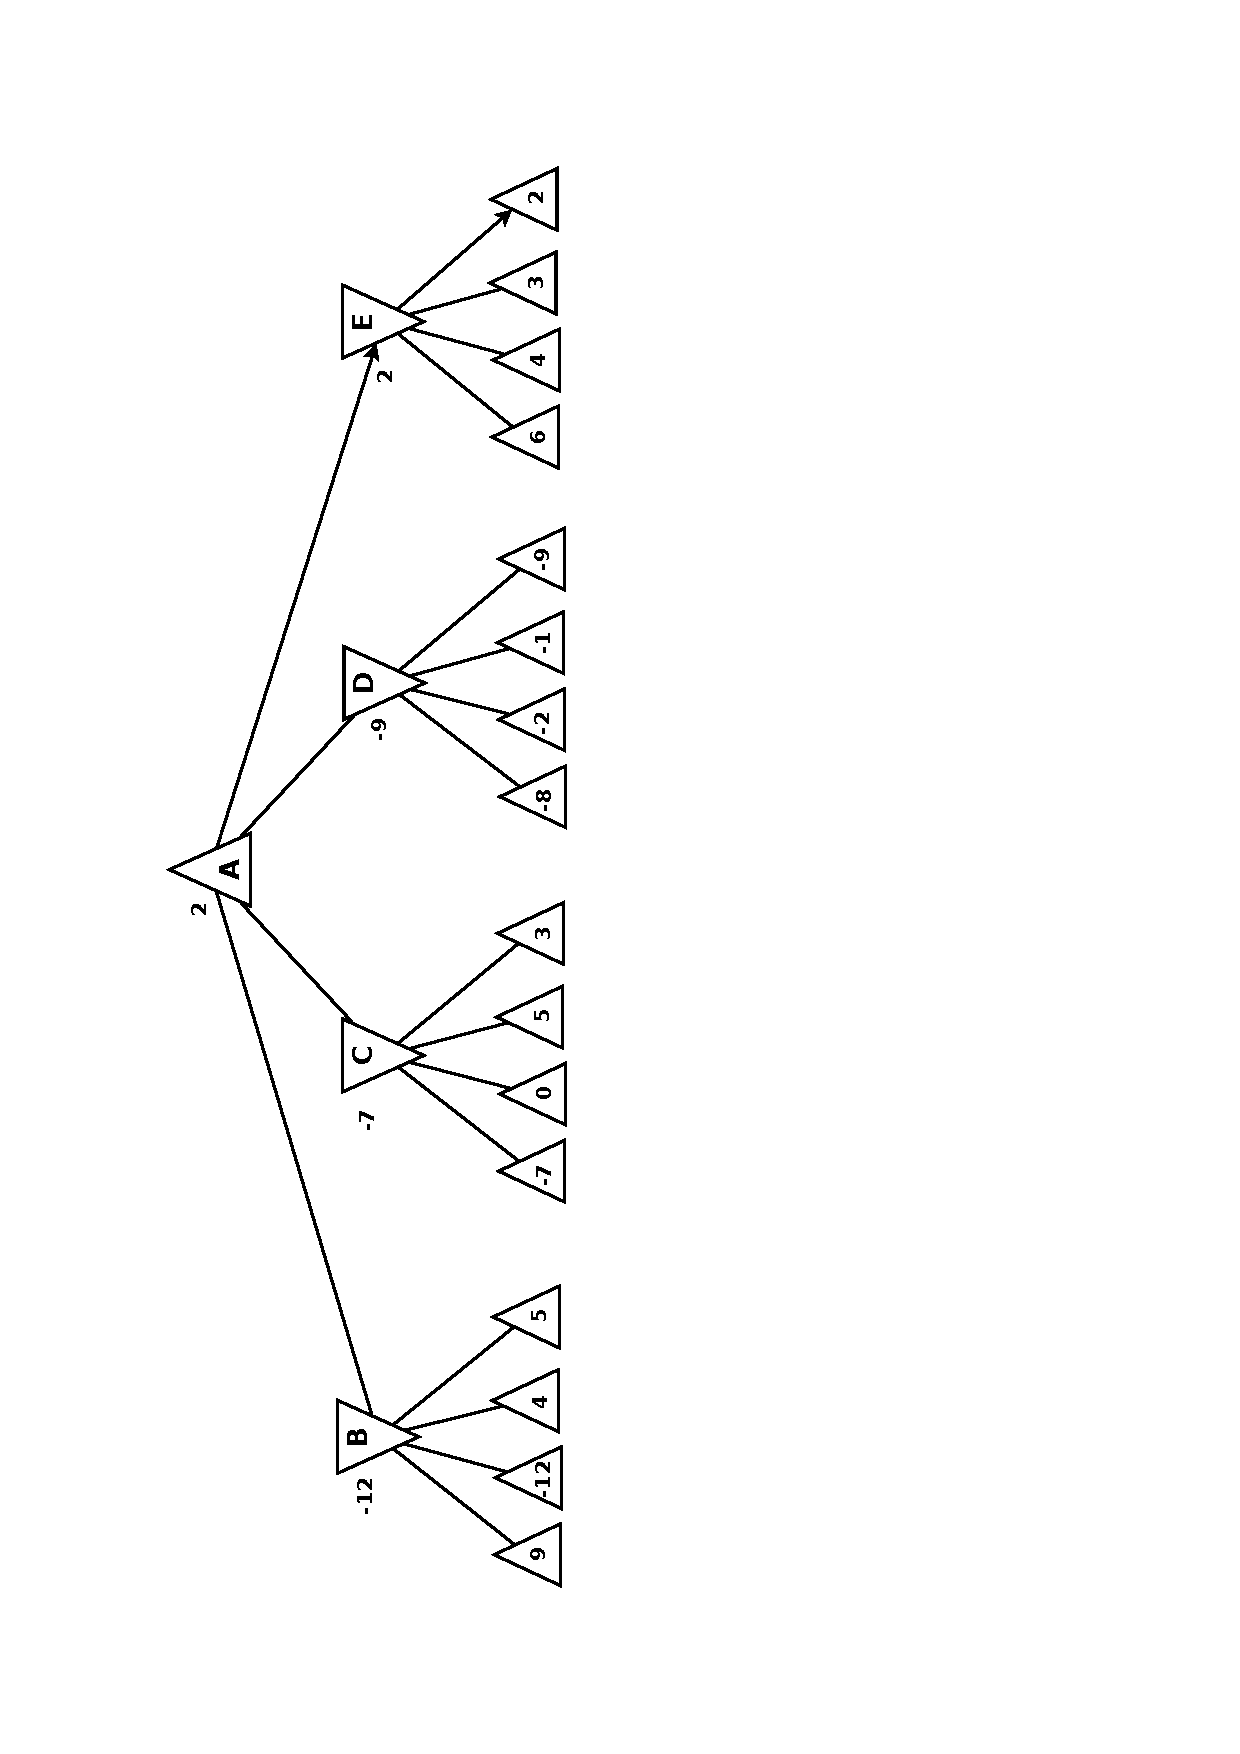
\includegraphics[width=0.3\textwidth, angle = -90, trim = 25mm 25mm 110mm 25mm,clip=true]{images/exercise1.pdf}}
\caption{The complete game tree of exercise 1. The $\bigtriangleup$ nodes represent MAX ones, whereas the $\bigtriangledown$ nodes represent MIN ones. The terminal nodes (leaves) show the utility values for MAX, whilst the other nodes are labeled with their minimax values.}
\label{fig:exercise1}
% Place the label just after the caption to make the link work
\end{figure} % table makes a floating object with a title